\section{\Bplus meson reconstruction}

In this section, the \Bplus and \PBzs mesons reconstruction strategy are presented. 
The schematic diagram of the workflow is shown in Fig.~\ref{fig:workflow}, starting from muons and tracks to \Bplus meson candidates. 
Muon candidates and tracks are required to pass several quality selection criteria as described in Section~\ref{sec:muonsel} and Section~\ref{sec:tracksel}. 
\Jpsi candidates are reconstructed by vertexing muon pairs with opposite charge, using {\footnotesize KinematicConstrainedVertexFitter}.
The \Bplus candidates are built by combining the \Jpsi candidates with each of the selected tracks.
Finally, a kinematic fit to the \Jpsi-$K^+$ system is performed, forcing the mass of dimuon pair to be equal to to the nominal \Jpsi mass based on PDG~\cite{PDG:2018}.
The selection criteria of the \Bplus candidates are described in Section~\ref{sec:Bsel}. \\

\begin{figure}[h]
\centering
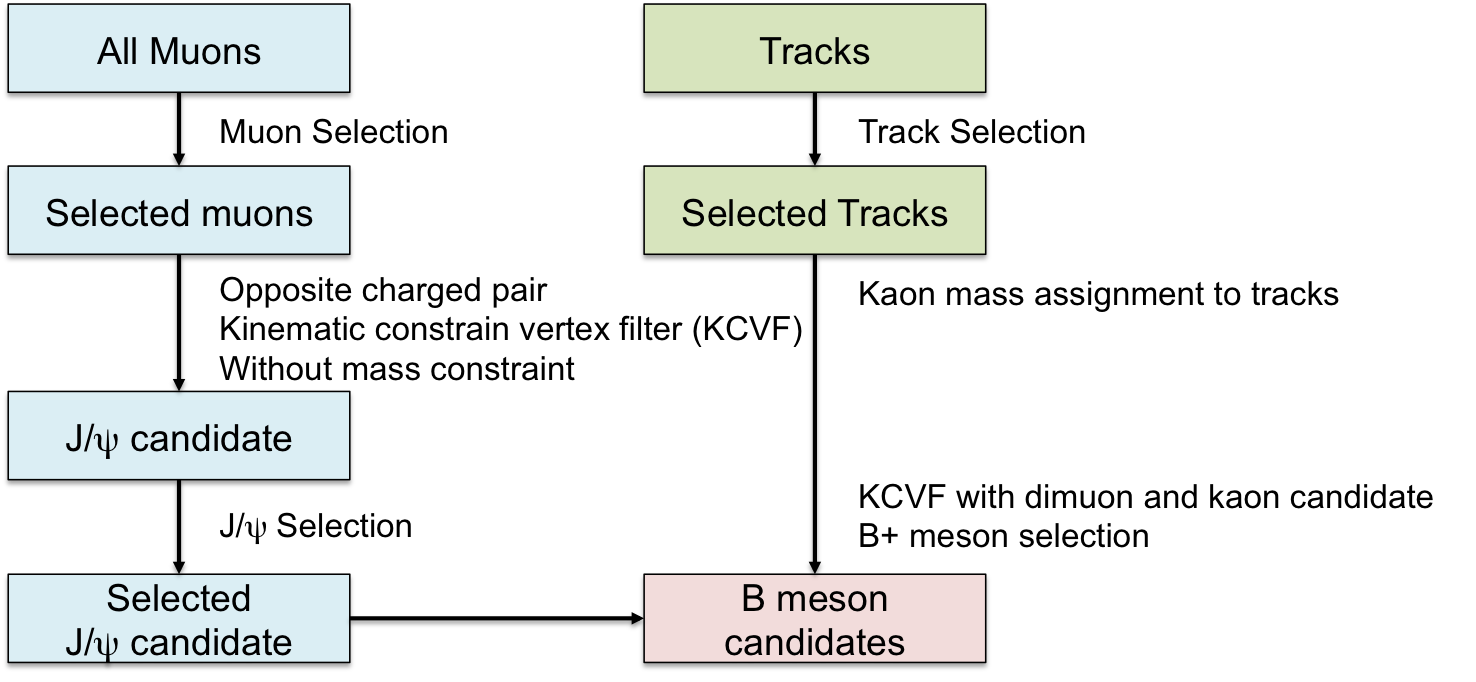
\includegraphics[width=0.9\textwidth]{Plots/BmesonReconstruction/BP.png}
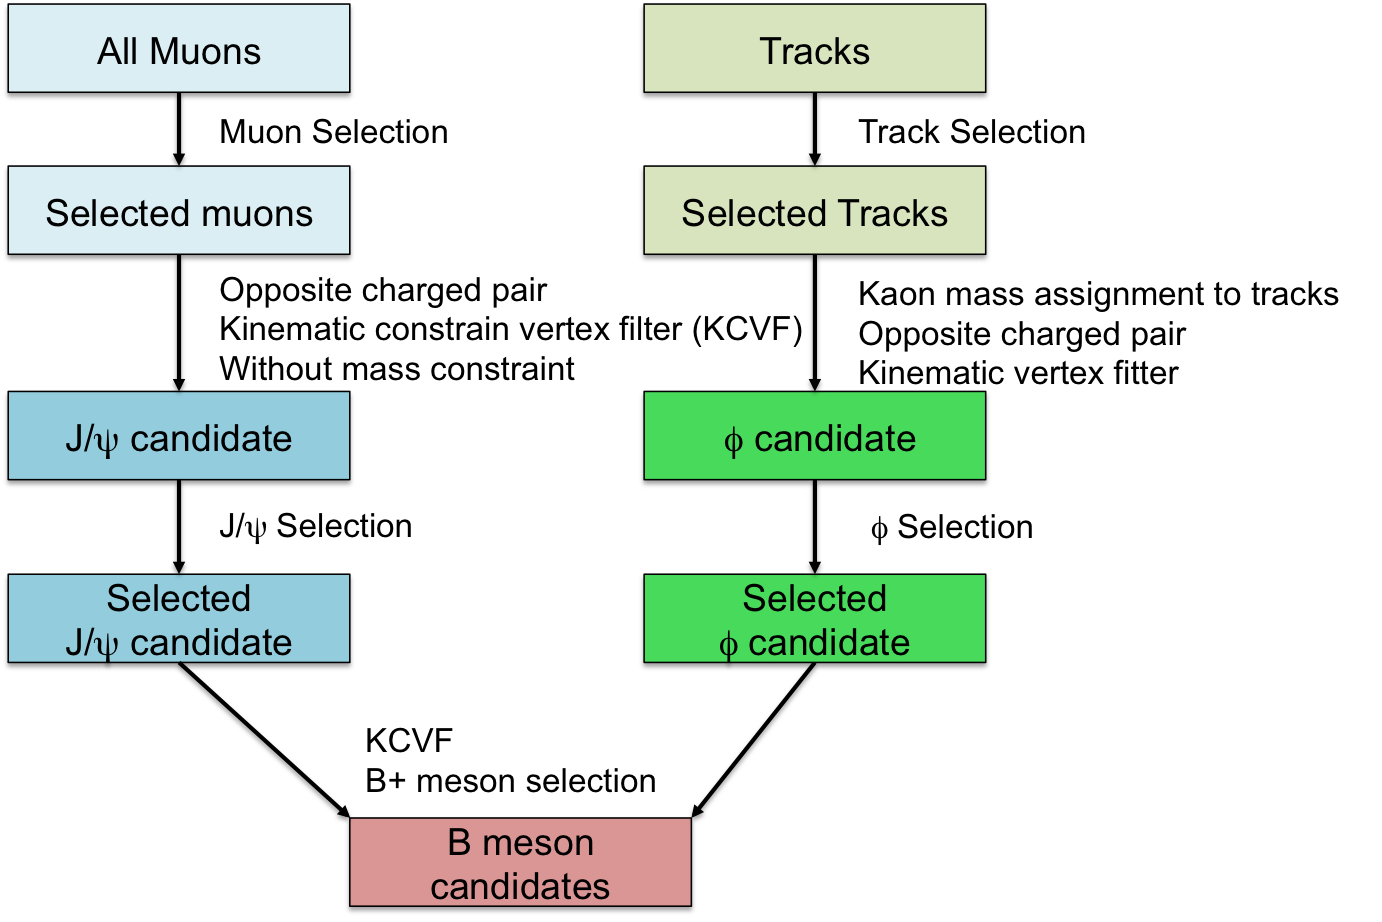
\includegraphics[width=0.9\textwidth]{Plots/BmesonReconstruction/Bs.png}
\caption{Schematic diagrams of the $B^+$ meson (top) and $B^0_s$ reconstruction workflows}
\label{fig:workflow}
\end{figure}


\subsection{Muon and \Jpsi selection}
\label{sec:muonsel}

The muon candidates are selected according to the {\it{hybrid-soft muon selection}}, developed for the muon analyses on the 2017 5.02\TeV data analyses~\cite{AN-16-048}. It is adapted from the soft-muon ID developed in the BPH group, with two modifications: a) the purity selection is removed, and b) the muon is required to be also global. 
The {\it{hybrid-soft muon selection}} includes the following cuts:
\begin{itemize}
\item \textit{isGlobalMuon} and \textit{isTrackerMuon};
\item \textit{isGoodMuon} $> 0$;
\item transverse impact parameter \textit{$\rm D_{xy}$} $< 0.3$;
\item longitudinal impact parameter \textit{$\rm D_{z}$} $< 20$;
\item \textit{nPixWMea} $> 0$ and \textit{nTrkWMea} $> 5$ (\textit{nPixWMea} and \textit{nTrkWMea} are  the number of pixel layers and strips, with valid hits, crossed by a single muon track)
\end{itemize}

Muons are also requested to fulfill the following acceptance selections:
\begin{equation}
\centering
\setlength\arraycolsep{20pt}
\begin{array}{l c r r}
\pt^{\PGm}>3.5\GeVc & & \text{for}\enspace \abs{\eta^{\PGm}}<1.2 & \\
\pt^{\PGm}>(5.77 - 1.89\times\abs{\eta^{\mu}})\GeVc & &  \text{for}\enspace 1.2\le\abs{\eta^{\PGm}}<2.1 &\\
\pt^{\PGm}>1.8\GeVc & & \text{for}\enspace 2.1\le\abs{\eta^{\PGm}}<2.4 &
\end{array}
\label{eq:SingleMuonAccCuts}
\end{equation}

Muons are required to match specific trigger of the following:
\begin{itemize}
\item \textit{Path: HLT$\_$HLT\_HIL1DoubleMu0\_v1}; \\
\item \textit{Last filter: hltL3f0L3Mu0L2Mu0DR3p5FilteredNHitQ10M1to5 $> 0$}.
\end{itemize}

This single muon selection is chosen in order to guarantee a reasonable (above $\approx10\%$) reconstruction and trigger efficiency for all the selected muons. %~\cite{AN-16-048}.

In addition to single muon quality selections, for a pair of muon candidates, the following selections are performed:
\begin{itemize}
\item the two muons have to have opposite sign;
\item dimuon invariant mass has to be within 0.15 GeV from the PDG \Jpsi mass;
\item probability of the two muon tracks to originate from the same decay vertex $>$ 1\%.
\end{itemize}


\subsection {Track selection}
\label{sec:tracksel}
%The track selection we applied are the same with $B^0_{s}$ AN~\cite{AN-19-055}.



Tracks were selected according to the following criteria, as recommended by the HIN tracking group:
\begin{itemize}
\item transverse momentum trkPt $> 0.2$, pseudorapidity $|\eta|$ $< 2.4$;
\item relative uncertainty on the track \pt, (trkPtError/trkPt) $< 0.1$;
\item sum of the numbers of Pixel and Strip hit $> 10$;
\item $\chi^2$ probability normalized by number of degrees of freedom and sum of the numbers of Pixel and Strip Layer hit $> 0.18$.
\end{itemize}

\subsection {$J/\psi$ and $\phi$ selection}

Finally, we also apply selections on the dimuon and dikaon tracks (for $B^0_s$ only):

\begin{itemize}
\item $|m_{\mu\mu} - m_{J/\psi}| < 0.15 GeV/c^{2}$
\item $|m_{K^{+}K^{-}} - m_{\phi}| < 0.015 GeV/c^{2}$
\end{itemize}




\clearpage
